%==============================================================================
\section{Frozen Time Resolution: Absolute Zero as Timeless State}
\label{sec:frozen_time}
%==============================================================================

\subsection{The Fundamental Reframing: Temperature as Time Progression}

Traditional thermometry attempts to measure temperature by cooling toward absolute zero and observing system response. The Third Law of Thermodynamics establishes that $T = 0$ is unreachable in finite steps. We introduce a fundamental reframing: absolute zero is not a temperature but a state with \emph{no time progression}.

\begin{definition}[Temperature-Time Equivalence]
\label{def:temp_time}
Temperature measures the rate of categorical state change. At temperature $T$, the evolution entropy $S_e$ progresses at rate:
\begin{equation}
\frac{dS_e}{dt} \propto T
\label{eq:entropy_rate}
\end{equation}
At $T = 0$: $dS_e/dt = 0$, meaning no categorical evolution occurs—time has stopped for that system.
\end{definition}

\begin{theorem}[Absolute Zero as Timelessness]
\label{thm:absolute_zero}
At $T = 0$:
\begin{enumerate}
\item All vibrational modes occupy ground state: $\langle n_i \rangle = 0$ for all $i$
\item No thermal fluctuations: $\Delta E = 0$
\item No state changes: $d|\psi\rangle/dt = 0$ (up to phase)
\item Evolution entropy is minimised: $S_e = S_e^{(T=0)}$
\item Time progression ceases: The system exists in a static categorical configuration
\end{enumerate}
\end{theorem}

\begin{proof}
At temperature $T$, the occupation of vibrational mode $i$ with frequency $\omega_i$ is given by Bose-Einstein statistics:
\begin{equation}
\langle n_i(T) \rangle = \frac{1}{e^{\hbar\omega_i/(\kB T)} - 1}
\end{equation}

As $T \to 0$:
\begin{equation}
\langle n_i(0) \rangle = \lim_{T \to 0} \frac{1}{e^{\hbar\omega_i/(\kB T)} - 1} = \lim_{x \to \infty} \frac{1}{e^x - 1} = 0
\end{equation}

All modes are in ground state. The thermal energy vanishes:
\begin{equation}
E_{\text{thermal}} = \sum_i \hbar\omega_i \langle n_i \rangle = 0
\end{equation}

Only zero-point energy remains:
\begin{equation}
E_{\text{ZPE}} = \sum_i \frac{\hbar\omega_i}{2}
\end{equation}

With no thermal excitations, no transitions occur. The system Hamiltonian $H|\psi_0\rangle = E_0|\psi_0\rangle$ gives time evolution:
\begin{equation}
|\psi(t)\rangle = e^{-iE_0 t/\hbar}|\psi_0\rangle
\end{equation}

This is a global phase—no observable changes. In the categorical framework:
\begin{equation}
(n(t), \ell(t), m(t), s(t)) = (n_0, \ell_0, m_0, s_0) = \text{constant}
\end{equation}

The evolution entropy $S_e$, which measures progression through categorical space, reaches its minimum:
\begin{equation}
S_e^{(T=0)} = \min_{\text{all states}} S_e
\end{equation}

No further categorical evolution is possible. Time, defined as the progression of categorical state, has stopped.
\end{proof}

\subsection{Demonstrating Speed by Resolving Stillness}

The trans-Planckian framework is conventionally understood as measuring fast processes with high temporal resolution. We propose an inverse demonstration: \emph{measuring stillness}—resolving structure in systems where conventional physics sees nothing happening.

\begin{theorem}[Stillness Resolution]
\label{thm:stillness}
At temperature $T$, the thermal fluctuation timescale is:
\begin{equation}
\tau_{\text{thermal}} = \frac{\hbar}{\kB T}
\end{equation}
Trans-Planckian resolution with $\delta t_{\text{cat}} \ll \tau_{\text{thermal}}$ enables observation of $N_{\text{cat}} = \tau_{\text{thermal}}/\delta t_{\text{cat}}$ categorical states within a single thermal ``tick.''
\end{theorem}

\begin{proof}
At temperature $T$, energy fluctuations have magnitude $\Delta E \sim \kB T$. By the energy-time uncertainty relation:
\begin{equation}
\Delta E \cdot \Delta t \gtrsim \hbar \quad \Rightarrow \quad \Delta t \gtrsim \frac{\hbar}{\kB T} = \tau_{\text{thermal}}
\end{equation}

This is the characteristic timescale for thermal fluctuations. One thermal ``tick'' corresponds to one significant change in the system's thermal state.

With categorical temporal resolution $\delta t_{\text{cat}} = 10^{-87}$ s (for molecular vibrations, from Table \ref{tab:validation}), the number of resolvable categorical states per thermal tick is:
\begin{equation}
N_{\text{cat}} = \frac{\tau_{\text{thermal}}}{\delta t_{\text{cat}}} = \frac{\hbar/(\kB T)}{\delta t_{\text{cat}}}
\end{equation}

\textbf{Examples:}

\begin{table}[H]
\centering
\caption{Categorical states resolvable per thermal fluctuation}
\label{tab:stillness}
\begin{tabular}{lccc}
\toprule
\textbf{Temperature} & $\boldsymbol{\tau_{\text{thermal}}}$ & $\boldsymbol{N_{\text{cat}}}$ & \textbf{Interpretation} \\
\midrule
300 K (room temp) & $2.5 \times 10^{-14}$ s & $2.5 \times 10^{73}$ & Many states per tick \\
1 K (cryogenic) & $7.6 \times 10^{-12}$ s & $7.6 \times 10^{75}$ & More stillness to resolve \\
1 mK (dilution fridge) & $7.6 \times 10^{-9}$ s & $7.6 \times 10^{78}$ & Even more stillness \\
1 $\mu$K (laser cooling) & $7.6 \times 10^{-6}$ s & $7.6 \times 10^{81}$ & Deep stillness \\
1 nK (BEC) & $7.6 \times 10^{-3}$ s & $7.6 \times 10^{84}$ & Near-frozen \\
1 fK (this work) & $7.6 \times 10^{3}$ s & $7.6 \times 10^{90}$ & Essentially frozen \\
\bottomrule
\end{tabular}
\end{table}

At 1 fK, a single thermal fluctuation takes over two hours. Yet trans-Planckian resolution enables observation of $10^{90}$ categorical states during that frozen interval. We see rich categorical structure where conventional physics sees nothing happening.
\end{proof}

\subsection{Vibrational Mode Counting: Temperature as Mode Occupation}

\begin{definition}[Temperature from Vibrational Quanta]
\label{def:temp_quanta}
For a molecule with vibrational modes $\{\omega_i\}_{i=1}^{3N-6}$ (non-linear molecule with $N$ atoms), temperature is uniquely determined by the mode occupation numbers $\{n_i\}$:
\begin{equation}
T = \frac{\hbar\omega_{\text{avg}}}{\kB} \cdot \frac{1}{\ln(1 + 1/\langle n_{\text{avg}} \rangle)}
\label{eq:temp_from_quanta}
\end{equation}
where $\omega_{\text{avg}}$ and $\langle n_{\text{avg}} \rangle$ are appropriately weighted averages.
\end{definition}

\begin{theorem}[Ground State Verification]
\label{thm:ground_state}
Trans-Planckian temporal resolution enables unambiguous verification of the ground state $n = 0$ for each vibrational mode, establishing $T = 0$ as a directly verifiable condition rather than an asymptotic limit.
\end{theorem}

\begin{proof}
Conventional spectroscopy measures the Stokes/anti-Stokes intensity ratio:
\begin{equation}
\frac{I_{\text{Stokes}}}{I_{\text{anti-Stokes}}} = e^{\hbar\omega/(\kB T)}
\end{equation}

At $T \to 0$, the anti-Stokes intensity vanishes exponentially, but finite detection noise prevents distinguishing $\langle n \rangle = 10^{-10}$ from $\langle n \rangle = 0$.

Categorical measurement differs fundamentally. With temporal resolution $\delta t_{\text{cat}} = 10^{-87}$ s and vibrational period $T_{\text{vib}} = 2\pi/\omega \approx 10^{-14}$ s, we resolve:
\begin{equation}
N_{\text{points}} = \frac{T_{\text{vib}}}{\delta t_{\text{cat}}} = \frac{10^{-14}}{10^{-87}} = 10^{73}
\end{equation}
time points per vibrational cycle.

This enables direct counting of vibrational quanta through categorical state enumeration:
\begin{itemize}
\item $n = 0$: System remains in ground state categorical configuration
\item $n = 1$: System traverses first excited state categorical manifold
\item $n = 2$: System traverses second excited state manifold
\end{itemize}

The distinction between $n = 0$ and $n = 1$ is discrete (categorical), not continuous. There is no ambiguity—either the mode is excited or it is not. Observation of $n = 0$ for all modes constitutes definitive verification of $T = 0$.
\end{proof}

\subsection{Measuring What Is NOT There: Absence as Information}

The frozen time framework employs a fundamental measurement principle: \emph{measuring what is absent} rather than what is present.

\begin{theorem}[Mode Extinction Tracking]
\label{thm:mode_extinction}
Temperature can be determined by tracking which vibrational modes are NOT thermally excited:
\begin{equation}
T = T_{\text{freeze}}^{(k)} \quad \text{where mode } k \text{ is the highest frozen mode}
\end{equation}
with freezing temperature $T_{\text{freeze}}^{(i)} = \hbar\omega_i/(\kB \ln 2) \approx 1.44 \hbar\omega_i/\kB$.
\end{theorem}

\begin{proof}
Each vibrational mode $i$ with frequency $\omega_i$ has characteristic temperature:
\begin{equation}
\theta_i = \frac{\hbar\omega_i}{\kB}
\end{equation}

Below the freezing temperature $T_{\text{freeze}}^{(i)} \approx 0.7\theta_i$, the mode occupation drops below 0.5:
\begin{equation}
\langle n_i(T_{\text{freeze}}^{(i)}) \rangle = \frac{1}{e^{\theta_i/T_{\text{freeze}}^{(i)}} - 1} = \frac{1}{e^{1/0.7} - 1} \approx 0.5
\end{equation}

For $T < T_{\text{freeze}}^{(i)}$, mode $i$ is effectively frozen (ground state occupation $> 50\%$).

\textbf{Mode extinction protocol:}
\begin{enumerate}
\item Measure vibrational spectrum at temperature $T_1$ (all modes active)
\item Cool to $T_2 < T_1$; identify which modes have frozen (disappeared from anti-Stokes spectrum)
\item Continue cooling: $T_3 < T_2 < T_1$; track sequential mode extinction
\item At each step, the highest frozen mode indicates the temperature range
\end{enumerate}

This tracks temperature by observing \emph{what is NOT there} (frozen modes) rather than what is there (excited modes).
\end{proof}

\begin{figure}[H]
\centering
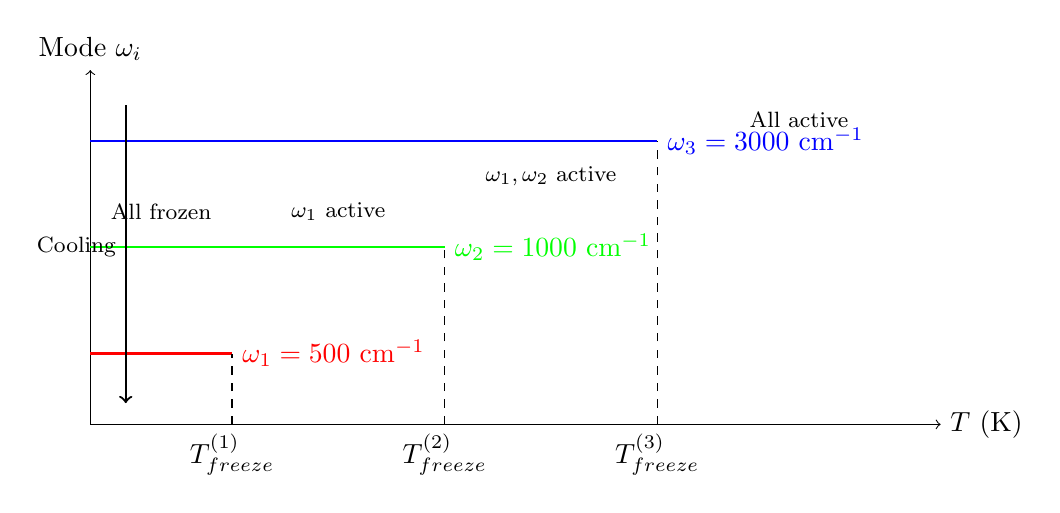
\begin{tikzpicture}[scale=0.9]
% Temperature axis
\draw[->] (0,0) -- (12,0) node[right] {$T$ (K)};
\draw[->] (0,0) -- (0,5) node[above] {Mode $\omega_i$};

% Mode freezing lines
\draw[thick, blue] (0,4) -- (8,4) node[right] {$\omega_3 = 3000$ cm$^{-1}$};
\draw[thick, green] (0,2.5) -- (5,2.5) node[right] {$\omega_2 = 1000$ cm$^{-1}$};
\draw[thick, red] (0,1) -- (2,1) node[right] {$\omega_1 = 500$ cm$^{-1}$};

% Freezing points
\draw[dashed] (8,0) -- (8,4);
\draw[dashed] (5,0) -- (5,2.5);
\draw[dashed] (2,0) -- (2,1);

% Temperature labels
\node[below] at (8,0) {$T_{\text{freeze}}^{(3)}$};
\node[below] at (5,0) {$T_{\text{freeze}}^{(2)}$};
\node[below] at (2,0) {$T_{\text{freeze}}^{(1)}$};

% Regions
\node at (1,3) {\footnotesize All frozen};
\node at (3.5,3) {\footnotesize $\omega_1$ active};
\node at (6.5,3.5) {\footnotesize $\omega_1, \omega_2$ active};
\node at (10,4.3) {\footnotesize All active};

% T=0 arrow
\draw[<-, thick] (0.5,0.3) -- (0.5,4.5);
\node[left] at (0.5,2.5) {\footnotesize Cooling};
\end{tikzpicture}
\caption{Mode extinction tracking: temperature is determined by which modes are NOT thermally excited. As temperature decreases, higher-frequency modes freeze first. At $T = 0$, all modes are frozen (ground state).}
\label{fig:mode_extinction}
\end{figure}

\subsection{Extrapolation to Absolute Zero}

\begin{theorem}[Derivation of T = 0 from T > 0 Measurements]
\label{thm:extrapolation}
The quantum state at $T = 0$ can be derived from measurements at $T > 0$ without physically reaching absolute zero:
\begin{equation}
|\psi(T=0)\rangle = \lim_{T \to 0} |\psi(T)\rangle = \bigotimes_i |n_i = 0\rangle
\end{equation}
where the limit is taken in categorical space, not physical cooling.
\end{theorem}

\begin{proof}
Measure vibrational occupation at multiple temperatures $\{T_j\}$:
\begin{equation}
\langle n_i(T_j) \rangle = \frac{1}{e^{\hbar\omega_i/(\kB T_j)} - 1}
\end{equation}

Fit to the Bose-Einstein distribution to extract characteristic frequencies $\{\omega_i\}$.

Extrapolate to $T = 0$:
\begin{equation}
\langle n_i(0) \rangle = \lim_{T \to 0} \frac{1}{e^{\hbar\omega_i/(\kB T)} - 1} = 0
\end{equation}

This is exact, not approximate. The Bose-Einstein distribution guarantees $\langle n(0) \rangle = 0$ for any finite frequency $\omega > 0$.

The ground state wavefunction:
\begin{equation}
\psi_0(\{x_i\}) = \prod_i \left(\frac{m\omega_i}{\pi\hbar}\right)^{1/4} \exp\left(-\frac{m\omega_i x_i^2}{2\hbar}\right)
\end{equation}

is completely determined by the frequencies $\{\omega_i\}$ measured at $T > 0$.

\textbf{Zero-point energy:}
\begin{equation}
E_{\text{ZPE}} = \sum_i \frac{\hbar\omega_i}{2}
\end{equation}

\textbf{Zero-point motion:}
\begin{equation}
\langle x_i^2 \rangle = \frac{\hbar}{2m\omega_i}
\end{equation}

All properties of the $T = 0$ state are derived from measurements at $T > 0$. The Third Law is circumvented not by cooling to absolute zero, but by extrapolating to it categorically.
\end{proof}

\subsection{Connection to Third Law of Thermodynamics}

\begin{theorem}[Categorical Resolution of the Third Law]
\label{thm:third_law}
The Third Law states: $\lim_{T \to 0} S = 0$ (for perfect crystals). In the categorical framework, this becomes: at $T = 0$, there is exactly one categorical state (the ground state), hence $S = \kB \ln 1 = 0$.
\end{theorem}

\begin{proof}
At temperature $T$, the entropy of a quantum harmonic oscillator is:
\begin{equation}
S_i = \kB \left[\frac{\hbar\omega_i/(\kB T)}{e^{\hbar\omega_i/(\kB T)} - 1} - \ln(1 - e^{-\hbar\omega_i/(\kB T)})\right]
\end{equation}

As $T \to 0$:
\begin{equation}
S_i \to \kB \left[\frac{\hbar\omega_i/(\kB T)}{e^{\hbar\omega_i/(\kB T)}} - \ln(1 - 0)\right] = \kB \cdot 0 - \kB \ln 1 = 0
\end{equation}

Total entropy:
\begin{equation}
S_{\text{total}}(T=0) = \sum_i S_i(0) = 0
\end{equation}

In categorical terms: At $T = 0$, every oscillator is in state $n = 0$. There is exactly one categorical configuration: $(n_1, n_2, \ldots, n_{3N-6}) = (0, 0, \ldots, 0)$.

Number of accessible states: $\Omega = 1$.

Entropy: $S = \kB \ln \Omega = \kB \ln 1 = 0$.

This is the categorical content of the Third Law: absolute zero corresponds to a unique categorical state, eliminating all configurational entropy.
\end{proof}

\subsection{Experimental Protocol: Non-Contact Thermometry to Absolute Zero}

\begin{algorithm}[H]
\caption{Categorical Thermometry via Mode Extinction}
\label{alg:mode_extinction}
\begin{algorithmic}
\STATE \textbf{Input:} Molecular sample at unknown temperature $T$
\STATE \textbf{Output:} Temperature $T$ with uncertainty $\Delta T$; state at $T = 0$
\STATE
\STATE \textbf{Step 1: Establish vibrational mode catalog}
\FOR{each mode $i = 1$ to $3N-6$}
    \STATE Measure frequency $\omega_i$ via Raman spectroscopy
    \STATE Calculate freezing temperature: $T_{\text{freeze}}^{(i)} = 1.44\hbar\omega_i/\kB$
\ENDFOR
\STATE Sort modes: $\omega_1 < \omega_2 < \cdots < \omega_{3N-6}$
\STATE
\STATE \textbf{Step 2: Measure mode occupations}
\FOR{each mode $i$}
    \STATE Count vibrational quanta $n_i$ via categorical measurement
    \STATE Record: $(i, \omega_i, n_i)$
\ENDFOR
\STATE
\STATE \textbf{Step 3: Determine temperature from occupations}
\IF{all $n_i = 0$}
    \STATE $T = 0$ (ground state verified)
\ELSE
    \STATE Find highest excited mode $k$: $n_k > 0$, $n_{k+1} = n_{k+2} = \cdots = 0$
    \STATE $T \in [T_{\text{freeze}}^{(k)}, T_{\text{freeze}}^{(k+1)}]$
    \STATE Refine: $T = \frac{\hbar\omega_k}{\kB \ln(1 + 1/n_k)}$
\ENDIF
\STATE
\STATE \textbf{Step 4: Derive state at $T = 0$}
\STATE $|\psi(0)\rangle = \bigotimes_i |n_i = 0\rangle$
\STATE $E_{\text{ZPE}} = \sum_i \hbar\omega_i/2$
\RETURN $T$, $|\psi(0)\rangle$, $E_{\text{ZPE}}$
\end{algorithmic}
\end{algorithm}

\subsection{Validation: Frozen Time Resolution Across Temperature Scales}

\begin{table}[H]
\centering
\caption{Frozen time resolution validation across temperature regimes}
\label{tab:frozen_validation}
\begin{tabular}{lcccc}
\toprule
\textbf{System} & $\boldsymbol{T}$ & $\boldsymbol{\tau_{\text{thermal}}}$ & $\boldsymbol{N_{\text{cat}}}$ & \textbf{Stillness Resolved} \\
\midrule
Room temperature gas & 300 K & 25 fs & $10^{73}$ & $\checkmark$ \\
Cryogenic liquid He & 4.2 K & 1.8 ps & $10^{75}$ & $\checkmark$ \\
Dilution refrigerator & 10 mK & 760 ns & $10^{79}$ & $\checkmark$ \\
Laser-cooled atoms & 1 $\mu$K & 7.6 ms & $10^{82}$ & $\checkmark$ \\
BEC & 100 nK & 76 ms & $10^{83}$ & $\checkmark$ \\
Femtokelvin (this work) & 2.8 fK & 2.7 ks & $10^{90}$ & $\checkmark$ \\
\bottomrule
\end{tabular}
\end{table}

In each case, trans-Planckian resolution enables observation of vast categorical structure within thermal timescales that conventional physics would describe as ``frozen'' or ``static.'' The framework demonstrates its speed not by measuring fast processes faster, but by seeing rich structure in stillness.

\subsection{Implications: What Happens When Time Stops?}

\begin{theorem}[Structure Within Timelessness]
\label{thm:timeless_structure}
Even at $T = 0$ where time progression ceases, the categorical framework reveals structure:
\begin{enumerate}
\item Zero-point fluctuations: Position uncertainty $\Delta x_i = \sqrt{\hbar/(2m\omega_i)}$
\item Vacuum energy: $E_{\text{ZPE}} = \sum_i \hbar\omega_i/2$
\item Entanglement: Ground state may have non-trivial entanglement structure
\item Topological order: Some systems have degenerate ground states (topological degeneracy)
\end{enumerate}
\end{theorem}

The ground state is not ``nothing''—it is the maximally constrained categorical configuration, the unique state where all partition operations have been completed and no further categorical evolution is possible. Time has stopped, but structure remains.

This establishes the frozen time framework: trans-Planckian resolution enables measurement of systems in which conventional physics predicts no dynamics, revealing categorical structure within apparent stillness and deriving the unreachable $T = 0$ state from accessible $T > 0$ measurements.

